%!TEX program = xelatex
\documentclass[10pt]{article}
\author{He Haoyu}
\usepackage{amssymb}
\usepackage{amsmath}
\usepackage{mathrsfs}
\usepackage{titlesec}
\usepackage{xcolor}
%\usepackage[shortlabels]{enumitem}
\usepackage{enumerate}
\usepackage{bm}
\usepackage{tikz}
\usepackage{listings}
\usetikzlibrary{arrows}
\usepackage{subfigure}
\usepackage{graphicx,booktabs,multirow}
\usepackage[a4paper]{geometry}
\usepackage{upquote}
\usepackage{float}
\usepackage{pdfpages}

\geometry{verbose,tmargin=2cm,bmargin=2cm,lmargin=2cm,rmargin=2cm}
\geometry{verbose,tmargin=2cm,bmargin=2cm,lmargin=2cm,rmargin=2cm}
\lstset{language=Matlab}
\lstset{breaklines}

\input defs.tex

\newtheorem{proposition}{Proposition}
\newtheorem{remark}{Remark}



\begin{document}

\date{\today}
\title{Introduction to Machine Learning, Spring 2022 \\
Homework 2\\
\small (Due Friday, Apr. 8 at 11:59pm (CST))}
\maketitle


\section{Problem1}
Given a set of data $\{(x_1, y_1), (x_2, y_2), \cdots, (x_N, y_N)\}$, where $y_i \in \{0, 1\}$. We want to conduct a binary classification, and the decision boundary is $\beta_0 + x^T\beta = 0$. When $\beta_0 + x^T\beta > 0$, the sample will be classified as 1, and 0 otherwise. 

\begin{enumerate}

\item[(a)]
Define a function which enables to map the range of an arbitrary linear function to the range of a probability {\color{red} [2 points]}\\

\item[(b)]
Derive the posterior probability of $P(y_i=1 | x_i)$ and $P(y_i=0 | x_i)$ {\color{red} [3 points]}\\

\item[(c)]
Write the log-likelihood for N observations, which means:
$$l(\theta) = logP(Y|X) = \sum_{i=1}^Nlog(P(y_i|x_i))$$
(Using the expression of $P(y_i|x_i)$ in (b) and eliminate redundant items) {\color{red} [5 points]}\\
\textbf{Solution:}

  \item[\textbf{(a)}]
      We can define  a map $f(x)=\frac{e^x}{e^x+1}$ from the range of an arbitrary linear function to the range of a probability
	\item[\textbf{(b)}] 
      Let $$\log \frac{P(y_i=1|x_i)}{1 - P(y_i=1|x_i)} = \log \frac{P(y_i=1|x_i)}{P(y_i=0|x_i)} =\beta_0 +x^T \beta$$
      By the properties of possibility, we know $$P(y_i=1|x_i)+P(y_i=0|x_i) = 1$$
      Thus,$$P(y_i=1|x_i) = \frac{\exp (\beta_0+x^T\beta)}{1+\exp (\beta_0+x^T\beta)}$$
      $$P(y_i=0|x_i) = \frac{1}{1+\exp (\beta_0+x^T\beta)}$$
	\item[\textbf{(c)}] 
      Let $\theta  = \{\beta_0,\beta\}$
      $$
      \begin{aligned}
          l(\theta) &= \log P(Y|X;\theta)
          \\&= \sum_{i=1}^N\log (P(y_i|x_i;\theta))
          \\&=\sum_{i=1}^N(y_i\log (P(y_i=1|x_i;\theta))+ (1-y_i)\log (P(y_i=0|x_i;\theta)))
          \\&=\sum_{i=1}^N(y_i(\beta_0+x^T\beta -\log (1+\exp (\beta_0+x^T\beta))))
      \end{aligned}
      $$
\end{enumerate}
\newpage
\section{Problem2}

\begin{enumerate}
    \item[(a)] 
    Given a random variable $X$ and its probability distribution is shown in Table 1. Now, we sample 8 times and get the results $\{3,1,3,0,3,1,2,3\}$. Please derive the MLE estimate for $\theta$($0 < \theta < \frac{1}{2}$). {\color{red} [4 points]} \\
    \begin{table}[t]
      \caption{probability distribution for $X$}
      \label{table1}
      \centering
      \begin{tabular}{c|c|c|c|c}
        \hline
        $X$ & 0 & 1 & 2 & 3 \\ \hline
        $P$ & $\theta^{2}$ & $2\theta(1-\theta)$ & $\theta^{2}$ & $1-2\theta$ \\
        \hline
      \end{tabular}
    \end{table}
    
    \item[(b)]
    Now we discuss Bayesian inference in coin flipping. Let's denote the number of heads and the total number of trials by $N_1$ and $N$, respectively. Please derive the MAP estimate based on the following prior:
    \begin{align*}
        p(\theta)=\left\{\begin{array}{ll}
        0.5 & \text { if } \theta=0.5 \\
        0.5 & \text { if } \theta=0.3 \\
        0   & \text { otherwise,}
        \end{array}\right.
    \end{align*}
    which believes the coin is fair, or is slightly biased towards tails. {\color{red} [4 points]} \\
    
    \item[(c)]
    Suppose the true parameter is $\theta = 0.31$. Please compare the prior in (b) with the Beta prior distribution(You can review this part in Lecture 07). Which prior leads to a better estimate when $N$ is small? Which prior leads to a better estimate when N is large? {\color{red} [2 points]} \\

\end{enumerate}
\newpage
\section{Problem3}
According to the following Fig.~\ref{fig2}, answer the following questions:
\begin{enumerate}
    \item[(a)]
    use the D-separation to discus whether the following statements are true or not: 
    \begin{itemize}
        \item[(1)] Given $x_4$, $ \{x_1, x_2\} $ and $ \{x_6, x_7\} $ are conditionally independent.{\color{red} [1(reason)+1(conclusion) points]}
        
		\item[(2)] Given $x_6$, $ x_3 $ and $ x_2 $ are conditionally independent.{\color{red} [1(reason)+1(conclusion) points]}
    \end{itemize}

	\item[(b)] if all the nodes are observed and boolean variables, please complete the process of learning the parameter $ \theta_{x_6|i,j} $ by using \textbf{MLE}, where $ \theta_{x_6|i,j} = p(x_6 = 1\mid x_3 = i, x_4 = j), i,j \in \{ 0, 1\}$.{\color{red} [6 points]}

	\begin{figure}[h!] 
		\centering
		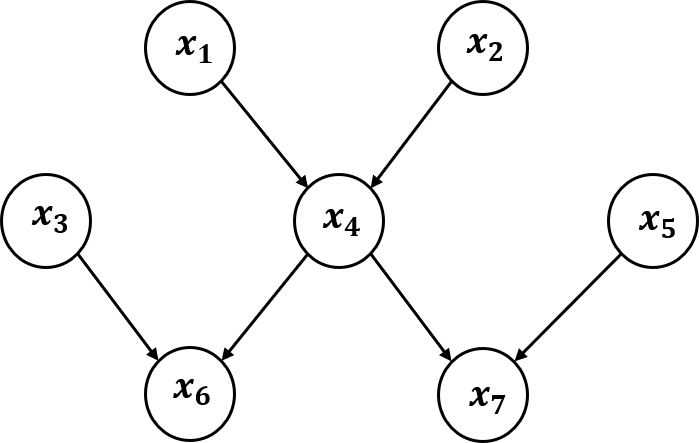
\includegraphics[width=2.5in]{3.png}
		\label{fig2}
		\caption{The Bayesian network for questions $3$.}
	\end{figure}

\textbf{Solution:}
    \item[\textbf{(a)}]
      \begin{enumerate}
        \item[{(1)}]True.
        Let A = $\{x_1,x_2 \}$, B = $\{x_6,x_7 \}$,
        the path is like $A\rightarrow x_4 \rightarrow B$ head-to-tail.
        For given $x_4$, $x_4$ is blocked, which means $ \{x_1, x_2\} $ and $ \{x_6, x_7\} $ are conditionally independent given $x_4$.
        \item[{(2)}] False. First of all, $x_3\rightarrow x_6 \leftarrow x_4$ is head-to-head path,so for given $x_6$, $x_6$ is not blocked.
        Then, $x_2 \rightarrow x_4 \rightarrow x_6$ is head-to-tail path, $x_4$ is not blocked for not given $x_4$.
        Thus, Given $x_6$, $ x_3 $ and $ x_2 $ are not conditionally independent.
      \end{enumerate}
    \item[\textbf{(b)}]
      Suppose we observed N points.
      Let $\theta = \{\theta_{x_1}, \theta_{x_2}, \theta_{x_3}, \theta_{x_4}, \theta_{x_5}, \theta_{x_6|i,j}, \theta_{x_7|j} \}$
      $$
      \begin{aligned}
          \log P(D|\theta) &= \log \prod_{k=1}^N P(x_{1k},x_{2k},x_{3k},x_{4k},x_{5k},x_{6k},x_{7k}|\theta)
          \\&= \sum_{k=1}^N \log  (P(x_{1k}|\theta)+ P(x_{2k}|\theta)+ P(x_{3k}|\theta)+ P(x_{4k}|\theta)+ 
          P(x_{5k}|\theta)+ P(x_{6k}|x_3,x_4,\theta)+ P(x_{7k}|x_4,\theta))
      \end{aligned}
      $$
      $$\frac{\partial \log P(D|\theta)}{\partial \theta_{x_6}|i,j} = \sum_{k=1}^N \frac{\partial \log P(x_{6k}|x_3,x_4,\theta)s}{\partial \theta_{x_6}|i,j}$$
      Now define $I(\cdot)$ be the indicator variable, $I(\cdot)=1$ if and only if is $(\cdot)$ is right, and 0 for all other cases.
      Thus,
      $$\theta_{x_6}|i,j = \frac{\sum_{k=1}^N I(x_{6k} = 1,x_{3k}=i,x_{4k}=j)}{I(x_{3k}=i,x_{4k}=j)}$$

    \end{enumerate}


\end{document}
